\documentclass{article}
\usepackage{multicol}
\usepackage{geometry} 
\usepackage{indentfirst}
\geometry{a4paper,top=3cm,left=2cm,right=2cm,bottom=3cm}
\usepackage{graphicx}
\graphicspath{ {./} }
\usepackage{amsmath}
\usepackage[
backend=biber,
style=alphabetic,
sorting=ynt
]{biblatex}

\usepackage{hyperref}
\hypersetup{
    colorlinks=true,
    linkcolor=black,
    filecolor=magenta,     
    citecolor=blue,
    urlcolor=black,
    pdftitle={Overleaf Example},
    pdfpagemode=FullScreen,
    }

\addbibresource{resources.bib}


\begin{document}



\begin{titlepage}
\sloppy

\begin{center}
BABE\c S BOLYAI UNIVERSITY, CLUJ NAPOCA, ROM\^ ANIA

FACULTY OF MATHEMATICS AND COMPUTER SCIENCE

\vspace{4cm}

\Huge \textbf{Exploring the association between stroke and weather
conditions using Artificial Intelligence} 

\vspace{1cm}

\normalsize - Research Project -

\end{center}


\vspace{7cm}

\begin{flushright}
\Large{\textbf{Ploscar Andreea Alina}}
\end{flushright}

\vspace{4cm}

\begin{center}
2022-2023
\end{center}

\end{titlepage}

\pagenumbering{gobble}

\tableofcontents

\newpage

\section{Abstract}

The study presents a new approach for assessing the impact of weather conditions on stroke incidence, making use of artificial intelligence to find this correlation and predict a sudden increase in the incidence of strokes based on meteorological conditions such as differences in atmospheric pressure, temperature, atmospheric fronts.

\section{Introduction}
\normalsize Stroke was the second cause of death in Romania in 2016 \cite{Donkor:2018dg} and is a major cause of mortality worldwide. Patients hospitalized with stroke can be treated, but due the sudden appearance of stroke symptoms, these patients require immediate attention from healthcare professionals, as well as available operating rooms. This process would be more efficient if healthcare workers could be aware that the incidence of strokes in the area is expected to increase, thus they would organize the non-emergency cases and the operating rooms using this information. 
\subsection{Aim}
The aim of the study is to assess the correlation between weather conditions and stroke incidence in Transylvania, Romania. As weather conditions temperature, air pressure, atmospheric fronts, precipitations and differences in these values are taken into consideration when analysing the correlation. For a better understanding of the relationship, underlying conditions of patients are taken into consideration. As a limitation, the study does not assess the impact of personal stress factors on patients hospitalized with stroke. 

\subsection{Related Work}
\begin{itemize}

\item\large "A study of weekly and seasonal variation of stroke onset"\\

\normalsize The paper \cite{Wang:2002dg} is relevant to this study as it presents the relationship between seasons, week days, age and stroke incidents. The results show a significant weekly and seasonal variation in the occurrence of stroke and a negative dose response relationship between seasonal variations in occurrence and age. This may be caused by the significant impact that lifestyle has on the probability of a stroke, topic that will be further discussed in this study.\\

Structure:
\begin{itemize}
\item Abstract - short overview of the article, containing the problem description, the time interval, the geographical area where the study was conducted, the methods and the results
\item Introduction - presents results and limitations of existing studies and the aim of the study
\item Subjects and methods - geographical and meteorological details of the targeted area, data collection and statistical methods used
\item Results
\begin{itemize}
    \item population characteristics
    \item weekly variation of stroke occurrence and the effect of age
    \item seasonal variation of stroke occurrence and the effect of age
\end{itemize}
\item Discussion - compares the obtained results to other studies, presents conflicting results and gives possible explanations for them, conclusion
\item References - list of cited and related work
\end{itemize}
In this paper, references appear as a list in the last section, in the following format: authors (year) title journal volume:pages. When cited, the format is: (authors year).\\

Citations: 105\\
References: 73


\item\large "Weather as a Trigger of Stroke"\\

\normalsize The paper \cite{Jimenez-Condea:2008dg} analyses the relationship between daily meteorological conditions and daily as well as seasonal stroke incidence. The approach is closed to our study, as it takes into consideration daily meteorological conditions, not only seasonal ones. The results show little association between atmospheric pressure(AP) and stroke, but higher association between stroke and variations in atmospheric pressure. The variation was computed as the value of AP compared to the previous day. Our study will also take into consideration 3, 6 and 12 hours variations. 

Structure:
\begin{itemize}
\item Abstract - background, methods, results, conclusions
\item Introduction - presents results and limitations of existing studies and the aim of the study
\item Methods 
\begin{itemize}
\item Subjects - geographical, temporal and quantitative details of analysed data
\item Classification and Variables - classification of patients and types of strokes, recorded medical and meteorological data
\item Statistical Analysis - statistical methods used to analyse the data
\item Ethics - ethical guidelines
\end{itemize}
\item Results 
\begin{itemize}
    \item Descriptive Data
    \item Daily Incidence Analysis
    \item Seasonal Analysis
\end{itemize}
\item Discussion - compares the obtained results to other studies, presents strengths and limitations of the study, conclusion
\item Acknowledgements - collaborations
\item References - numbered list of cited and related work
\end{itemize}
In this paper, references appear as a numbered list in the last section, in the following format: authors title journal year;volume:pages. When cited, the format is: [number] representing index in references list.\\

Citations: 73\\
References: 34

\item\large "The association between weather conditions and stroke admissions in Turkey"\\

\normalsize \cite{Çevik:2015dg} is focused on data from turkey, area that is closer to the one covered by the present study, i.e. Romania, so the meteorological conditions will be more similar to the ones in our study. The paper takes into consideration ischemic stroke (IS), hemorrhagic stroke (HS) and subarachnoidal hemorrhage (SAH) and The results from this paper present no association between incidence of overall admissions due to strokes and meteorological parameters, but they do demonstrate an association between admissions due to SAH ans HS and weather conditions, especially temperature. 

Structure:
\begin{itemize}
\item Abstract - aim of the study, details about used data, results
\item Introduction - presents results and limitations of existing studies and the aim of the study
\item Materials and Methods 
\begin{itemize}
\item Study Design - geographical, temporal and quantitative details of analysed data, diagnosis details
\item Meteorological data - geographical and meteorological details about data
\item Statistical Analysis - statistical methods used to analyse the data
\end{itemize}
\item Results - explained results
\item Discussion - compares the obtained results to other studies, presents strengths and limitations of the study, conclusion
\item References - list of cited and related work
\end{itemize}
In this paper, references appear as a list in the last section, in the following format: authors (year) title journal volume:pages. When cited, the format is: (author year)\\

Citations: 24\\
References: 22

\item\large "An Improved Back Propagation Neural Network Model and Its Application"\\

\normalsize The article \cite{Fang:2014dg} approaches the problem of finding a relationship between stroke incidence and weather conditions using a back propagation neural network, method that is closer to the one further presented in the present study. The results are in line with the ones presented above, presenting a stronger relationship between stroke incidence and atmospheric pressure, and a weaker, negative relationship between stroke incidence and temperature.\\


Structure:
\begin{itemize}
\item Abstract - overview, aim of the study, details about used data, results
\item Introduction - background, short description about methods
\item Model imporvement
\begin{itemize}
\item Notations - legend of notations and their meanings
\item The BPNN Flow - figure of the BPNN presenting the layers, input, output
\item Forward Propagation Process of Signal - mathematical explanations for hidden and output layers
\item Back Propagation Process of Error - mathematical explanation of used formulas and functions
\item The Improved BPNN Algorithm - description of improvements
\item Other Network Parameters - list of parameters for BPNN and environment
\item Model Solution - details about training samples input, samples training, samples prediction and effect, results
\item Model evaluation and promotion - describing the model as a prediction method
\end{itemize}
\item Acknowledgments
\item References - numbered list of cited and related work 
\end{itemize}
In this paper, references appear as a list in the last section, in the following format: authors, title, journal, volume, no, pages, year. When cited, the format is: [number] representing index in references list\\

Citations: 4\\
References: 4

\item\large "Personalized Spiking Neural Network Models of Clinical and Environmental Factors to Predict Stroke"\\

\normalsize The paper \cite{Doborjeh:2022dg} proposes a new method for the identification of associations between clinical and environmental time series: spiking neural networks. This paper is relevant to the present study, as it uses machine learning methods and also takes into consideration individual and family related factors.\\

Structure:
\begin{itemize}
\item Abstract - background, purpose of the study, details about used data and methods, results
\item Introduction - medical and technical explanations, existing work and results, new approaches in this paper
\item Methods - description of method, notations, schemas, 
\begin{itemize}
\item Method and System for Personalized Predictive Modeling on Integrated Personal Clinical Data and Dynamic Data of Environmental Changes - in detail explanation of the method, charts for data visualisation, 
\item Encoding of Environmental Time‐Series Data - description of encoding method
\item Environmental Data Mapping into a Personalized SNN Model - description of data mapping, variables and dimensions
\item Unsupervised Learning in the PSNN Model - method description
\item Supervised Learning, Classification and Prediction - method description
\end{itemize}
\item Study Population and Datasets - details about involved data (quantitative, temporal, spatial, classifications by age, gender)
\item Results - explained results, charts, figures
\item Personalized Profiling of Individual Risk of Stroke Using Environmental Data
\item Discussion - compares the obtained results to other studies, presents the advancement made by the study
\item Conclusion - overview, future work
\begin{itemize}
    \item Acknowledgements
    \item Author Contribution
    \item Funding
\end{itemize}
\item Declarations - legal aspects
\begin{itemize}
    \item Ethics Approval
    \item Consent to Participate
    \item Conflict of Interest
    \item Open Access
\end{itemize}
\item References - numbered list of cited and related work
\end{itemize}
In this paper, references appear as a list in the last section, in the following format: authors, title, journal, volume, no, pages, year. When cited, the format is: [number] representing index in references list\\

Citations: 0\\
References: 0\\
Accesses: 411
\end{itemize}

\subsection{Original Contribution}

The present study adds value to the research in the medical and meteorological fields as it gives an answer to an important question: Can stroke incidence be predicted using weather conditions? The answer to this question would help healthcare professionals save more patients hospitalized with this health emergency, contributing to the decrease of mortality due to stroke. Especially in Romania, where the study is conducted, this would have a great impact on the healthcare system overall. In comparison to existing work, the study uses artificial intelligence: neural networks and clustering algorithms to find the specified correlation, is focused on a small area, Transylvania, Romania and uses data collected over nine years 2013-2021. 

\newpage
\section{Datasets} \label{datasets}
\subsection{Meteorological Data}
Numerical data is downloaded from Meteomanz.com and is collected from meteorological stations in Transylvania. The data contains collected values by days and by hours between Jan 2013 - Dec 2021. Data preprocessing includes formatting the values to be only numerical, removing redundant data. Because stroke incidence seems to be more related to the sudden differences in temperature and atmospheric pressure rather than their absolute values, these differences were computed using data collected by hours and added to the data by days dataset as columns for each line (day). The differences were computed for every 3 hours. For this process, the Pandas library from python was used. 

\subsection{Medical Data}

The medical dataset was collected by healthcare professionals in Cluj-Napoca, Cluj, Romania between 2013-2021 and contains annonymous records of patients admitted with strokes. These records present data about the exact time of the stroke, the place where the patient was located at that time, generic data about the patient: gender, age, underlying health conditions. 


\section{Methods}
\subsection{Meteorological Data Visualization}

To visualize the preprocessed meteorological data, the following libraries were used: Bokeh, Pandas, Matplotlib. The figures presented below represent the average values for temperature and atmospheric pressure over the studied time period and the 3 hours differences in these parameters.

\begin{figure*}[h!]
\begin{multicols}{2}
\centering
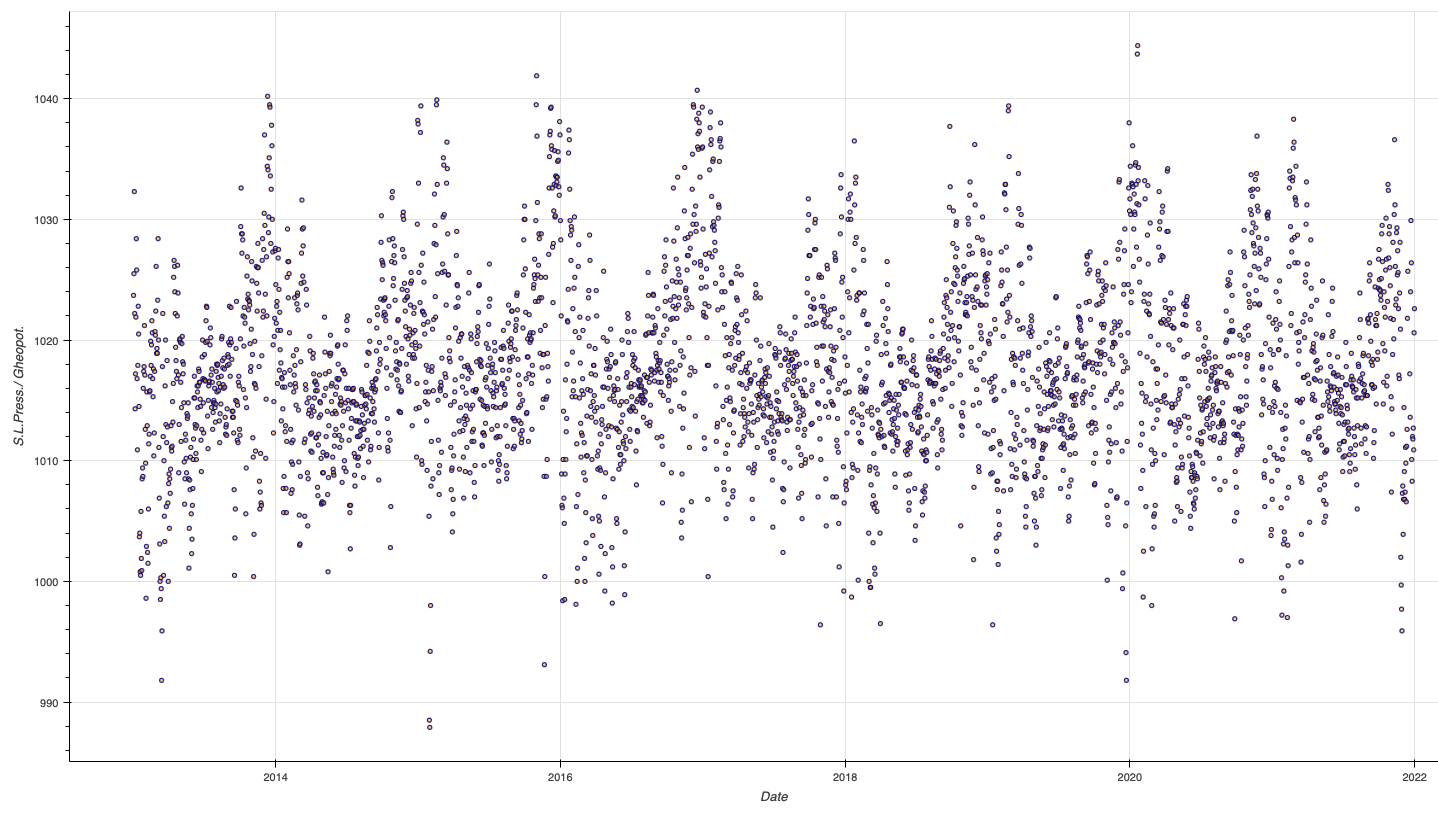
\includegraphics[width=6cm]{PressureAvg.png}
\caption{Average Atmospheric Pressure}

\centering
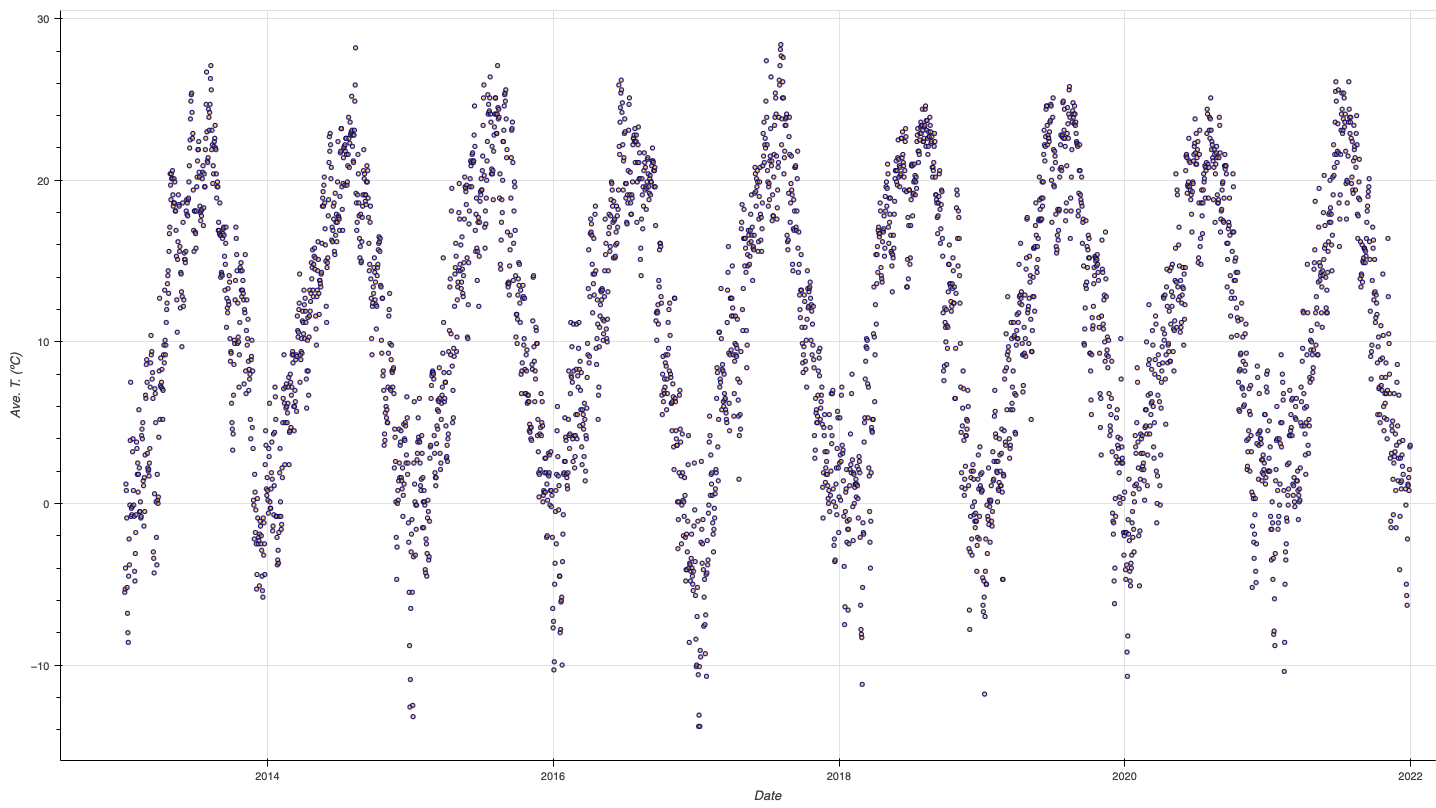
\includegraphics[width=6cm]{TempAvg.png}
\caption{Average Temperature}

\centering
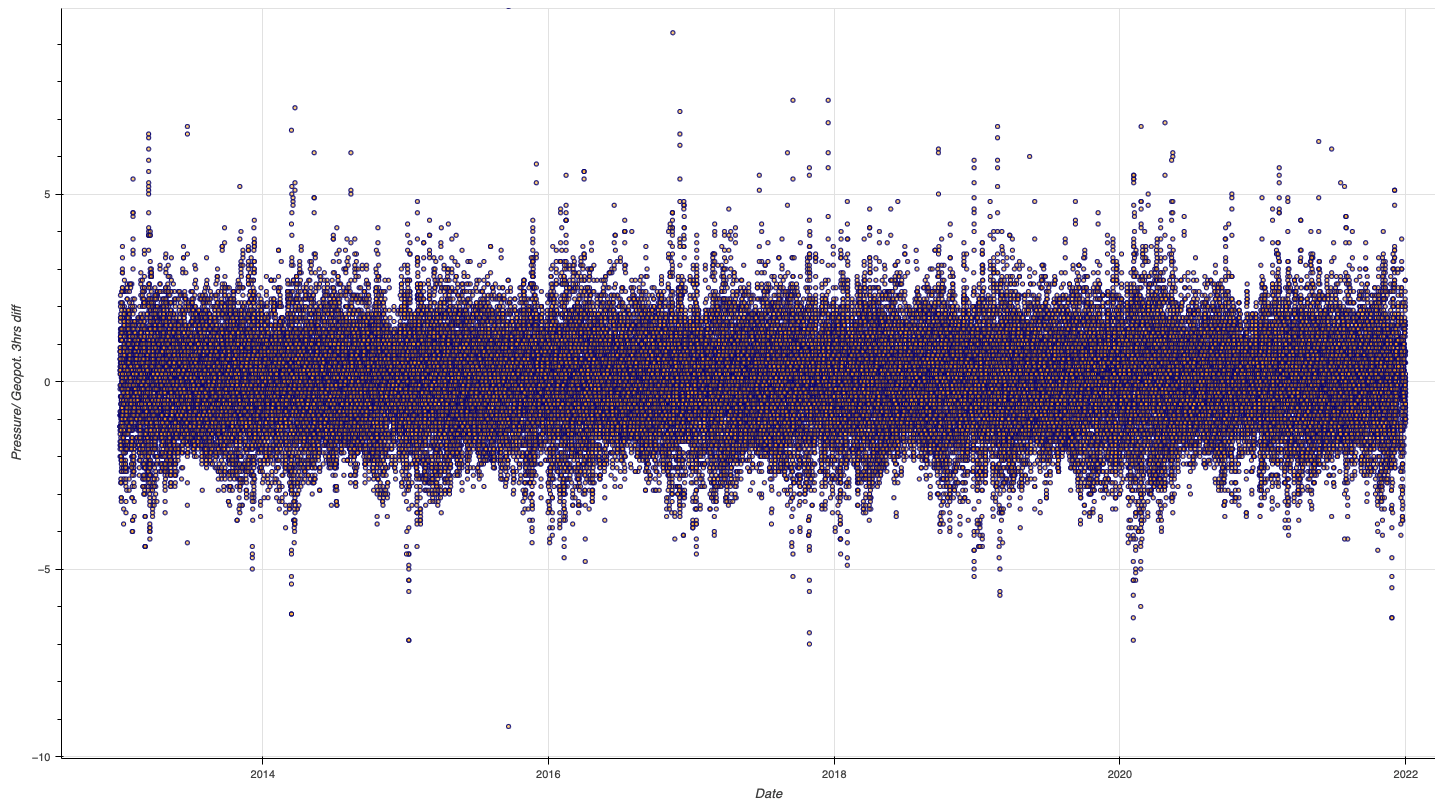
\includegraphics[width=6cm]{PressureDiff.png}
\caption{Atmospheric Pressure 3 hours Differences}

\centering
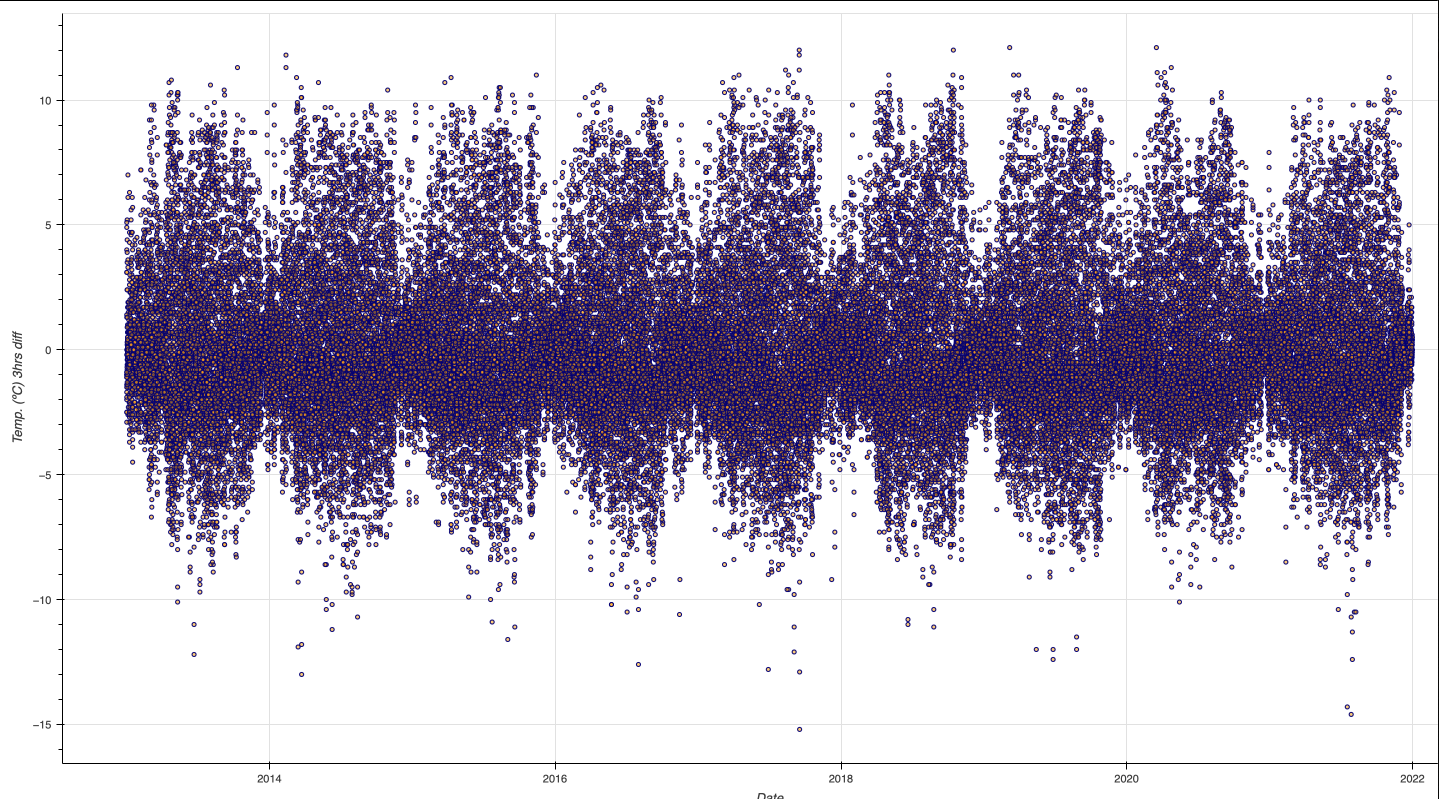
\includegraphics[width=6cm]{TempDiff.png}
\caption{Temperature 3 hours Differences}

\end{multicols}
\end{figure*}

\subsection{Medical data Clustering}

For grouping the data points representing patients, two clustering algorithms are used: K-Means Clustering and Mean-Shift Clustering. These unsupervised learning algorithms are used to identify groups of patients with similar features.

\subsubsection{K-Means Clustering}

\subsubsection{Mean-Shift Clustering}

\subsection{Identifying Variations}

Changes in the weather conditions are often times linked to atmospheric fronts passing over the area. Variations in weather parameters such as temperature and atmoshperic pressure can signal the passing of an atmoshperic front. These fronts can be classified into: cold front, warm front, stationary front and occluded front. Strokes incidence seems to be affected by variations in weather conditions, so identifying the moment a front passes over an area could lead to a prediction for stroke incidence. To verify this hypothesis, the maximum variations need to be first identified from the meteorological dataset. Two algorithms are used for this process: Feature Importance and Outliers Identification.

\subsubsection{Feature Importance}
\subsubsection{Outliers Identification}

\subsection{Neural Network}

The problem of predicting a sudden increase in the incidence of strokes  can be seen as a classification problem and a possible approach for this is using an artificial neural network. This ANN receives as input the weather conditions for a day and outputs 1 or 0, 1 if this day corresponds to an increase in stroke incidence, i.e. the conditions for this day match the previously learned model for days correlated to a larger number of patients admitted, 0 otherwise. 

\section{Experimental Modelling}

\subsection{Data}

To measure the performance of the algorithms and the validity of the hypothesis, multiple experiments are performed. The data is split into train, validate and test data. The train and validate data are used during the training phase of the algorithm, while the test data is used after the model is trained, to assess the obtained performance. The experiments are done using the validation data. Test data is used after the model is trained and the performance is assessed to manually test the algorithm, simulating its usage by an end user. 

Data is collected as described in \ref{datasets}. As medical data contains records of strokes that occurred in multiple cities of Romania, multiple weather stations must be 
taken into consideration during the experiments. Not all cities appearing in the medical records have a weather station, so the closest weather station will be taken into consideration. 


\subsection{Metrics} \label{metrics}

Although the model needs to perform well, as it would be used in medical facilities and could affect the performance of the medical system, a small type I error is accepted, i.e. the model could predict a spike in the incidence of stroke, but in reality there is no spike. In this case, the medical staff would be prepared for stroke emergencies, but this does not have a negative impact on their performance. A type II error would mean that the model predicted no increase, so the doctors would not prepare for a spike that does appear in reality. This type of error should be minimized as much as possible in the model.
\\

The following metrics are used for evaluating the experiments:
\begin{itemize}
    \item Accuracy - number of correct predictions over all predictions
    \item Precision - how many positive predictions are true positives
    \item Recall - how many of the positives were detected as positive
    \item F1-Score - harmonic mean of precision and recall
\end{itemize}
Because the recall and precision should be balanced, the F1-Score is the most meaningful for the purpose of this study. The recall should be maximized, but without dropping the precision to a small value.

Value references that would validate the model:
\begin{itemize}
    \item Accuracy $>$ 90\%
    \item Precision $>$ 77\%
    \item Recall $>$ 85\%
    \item F1-Score $>$ 80\%
\end{itemize}

\subsection{Formal Model}

Mathematically, the experiments require in the first step calculations of differences by hours of the following parameters, seen as variables: temperature (T), atmospheric pressure (AP), humidity (H), wind direction (WD), wind speed (WS). For this first computation the values for these parameters for each hour are used and 24 differences are computed for every day as follows: 
\\

For hour taking values from 0 to 24 and V being each one of the parameters (T, AP, H, WD, WS):

\begin{align}
    \begin{cases}
    E = (hour + 3) \% 24 \\
    S = hour \\
    V\_S-E = V\_E - V\_S 
\end{cases}
\end{align}

The Artificial Neural Network used in the experiment computes the loss using the Cross Entropy loss function:

\begin{equation}
     H(p,q)\ =\ -\sum _{i}p_{i}\log q_{i}\ =\ -y\log {\hat {y}}-(1-y)\log(1-{\hat {y}})
\end{equation}

The activation function used for the linear layers is ReLU:

\begin{equation}
f(x) = \begin{cases}
             x  & \text{if } x > 0 \\
             0  & \text{otherwise }
       \end{cases} 
\end{equation}


\section{Case study}

To illustrate the methodology and approach of the presented paper, a case study is performed using an initial, smaller dataset. For this, the medical and meteorological records from Cluj-Napoca city are taken into consideration. The experiment can then be extended to cover a larger area.

\subsection{Data processing}

Meteorological data is downloaded from Meteomanz.com, using the station code 15120, corresponding to Cluj-Napoca. The data covers the time interval 01.2013-12.2021. Medical data is collected from the public hospital in Cluj-Napoca and contains records from the same time interval.
\\

The data is processed using the Pandas python library. More processing is needed for meteorological data, as separate files are downloaded for data by days and data by hours. This information is aggregated to compute the 3 hours differences used further. The parameters taken into consideration are: temperature (T), atmospheric pressure (AP), humidity (H), wind direction
(WD), wind speed (WS). The medical records contain information about the day of the stroke occurrence, gender, age and medical history. Only 20\% of the records give information about the exact time of the stroke, so this information is not kept, as completing the rest of the records with generated data would only induce errors. The data is split into 2 categories: train and test. The training dataset contains records from 07.2013-12.2021 and the testing one from 01.2013-06.2014. 

\subsection{Data visualization}

\subsubsection{Meteorological Data}

Before applying the algorithm, data visualization was used to observe the days considered more probable to match with stroke occurrences. 

In the first trial we consider the temperature and pressure differences for every 3 hours as the main meteorological parameters and draw a 3D plot with these values over the full time interval. As the data in this plot (\ref{figure3D}) is not easily readable, a 2D plot with color gradient is also made (\ref{figure2DColor}). 

\begin{figure}[ht] 
\centering
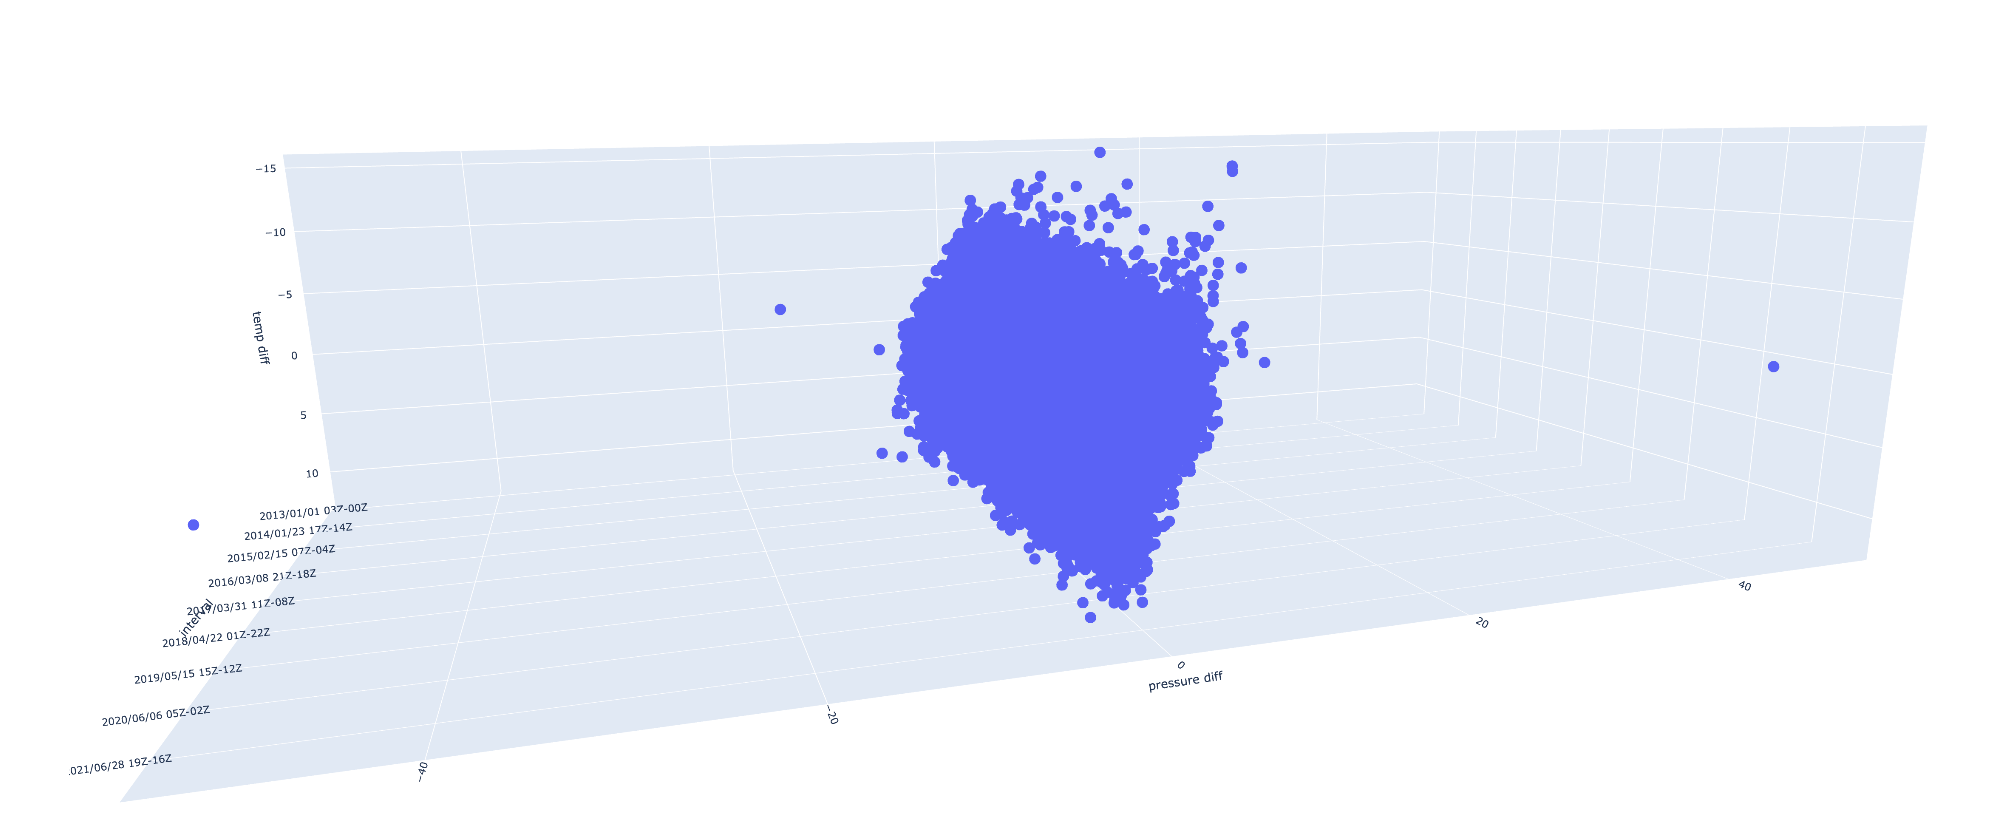
\includegraphics[height=7cm]{3dPlot.png} 
\caption{3D plot of meteorological data}
\label{figure3D}
\end{figure}

\begin{figure}[h!] 
\centering
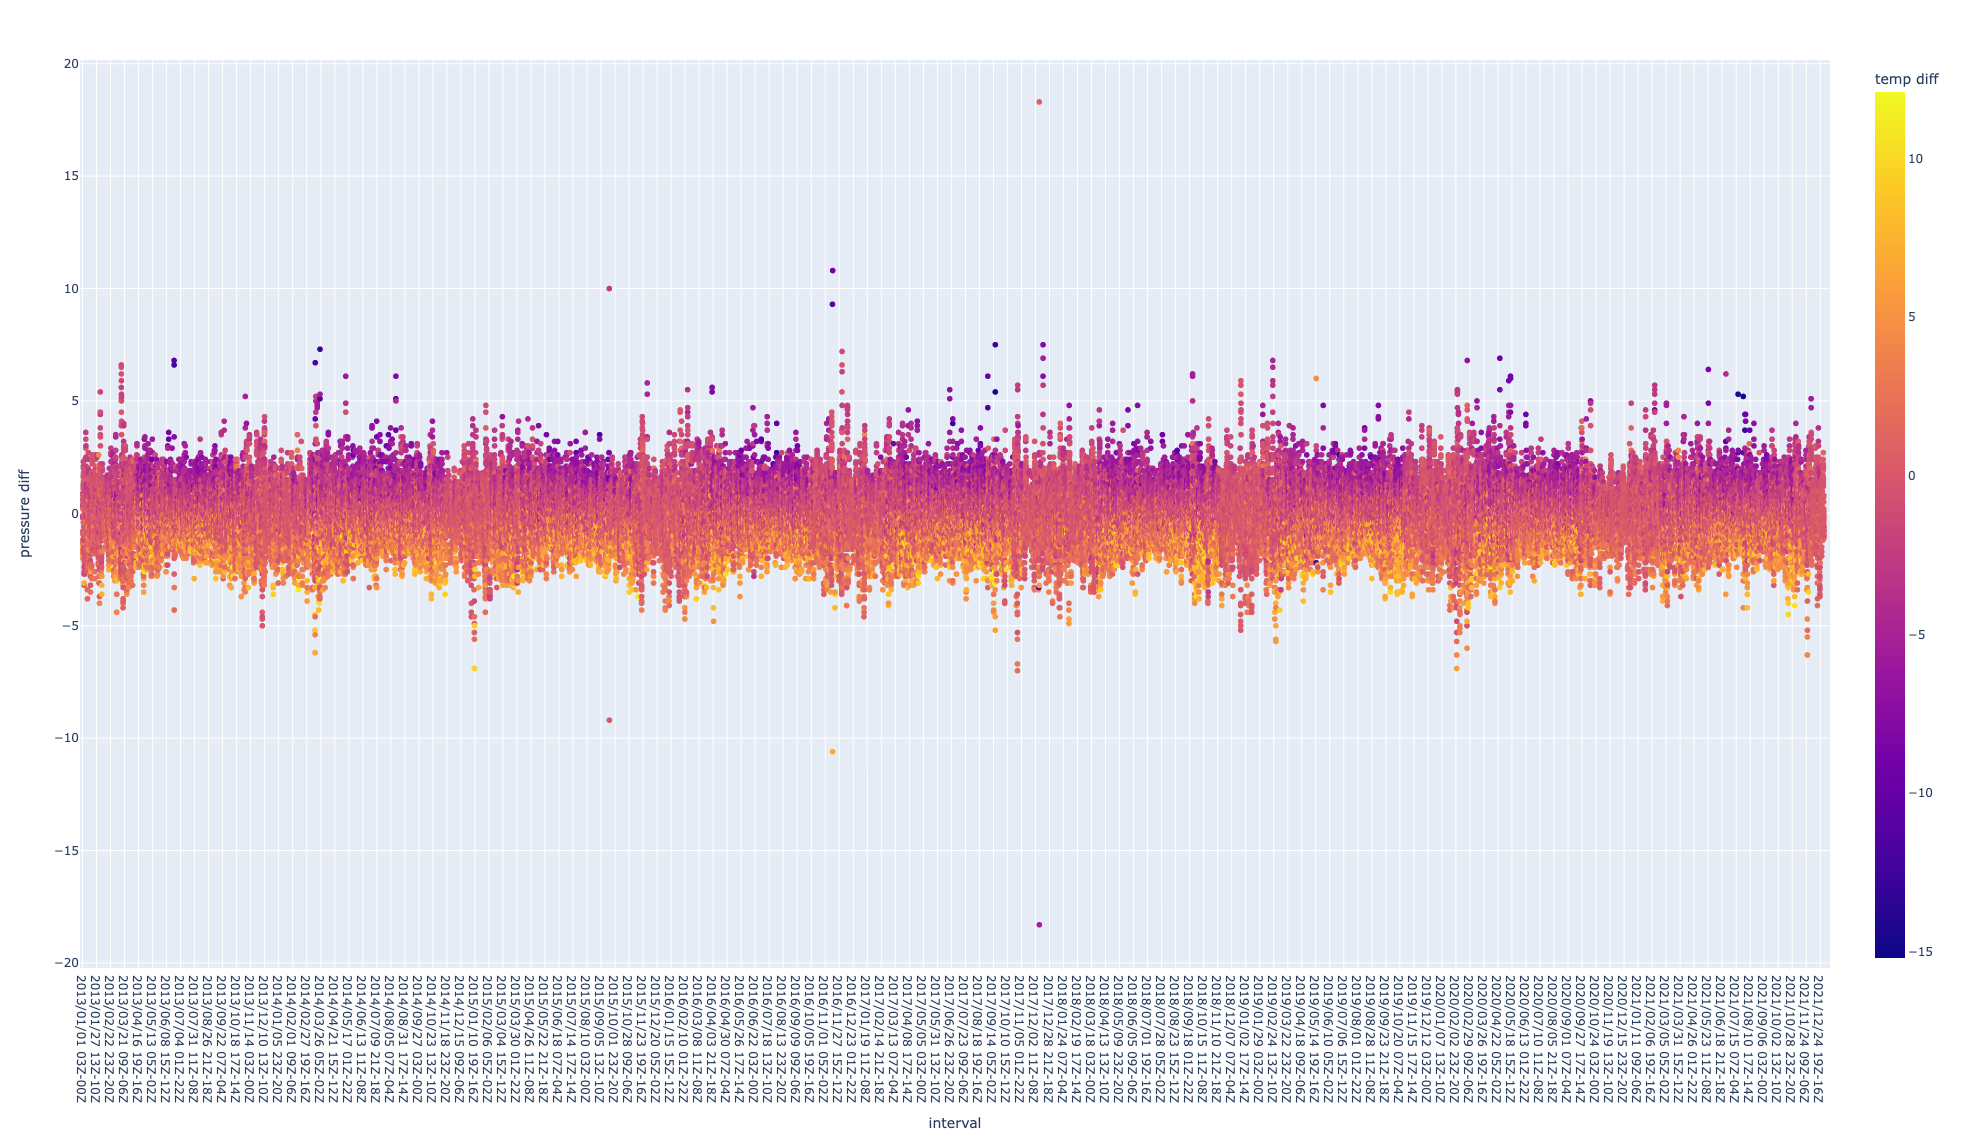
\includegraphics[height=9cm]{newplot (1).png}
\caption{2D plot of meteorological data} 
\label{figure2DColor}
\end{figure}

\newpage

The visual result matches the expected one, some days across the time interval have greater temperature and pressure differences and a possible negative relationship between these two parameters can be observed. Most points with a larger, positive difference in pressure have a negative difference in temperature and the other way around. Most of the point are located in the [-2.5, 2.5] interval on the pressure diff axis, so these values will be considered normal. A few points are located above 10 or below -10, these values will be omitted as there is a high probability they are errors. The values in the intervals [-10, -2.5] and [2.5, 10], represented in Figures \ref{interval1} and \ref{interval2} will be analysed further.

\begin{figure*}[h!] 
\begin{multicols}{2}

\centering
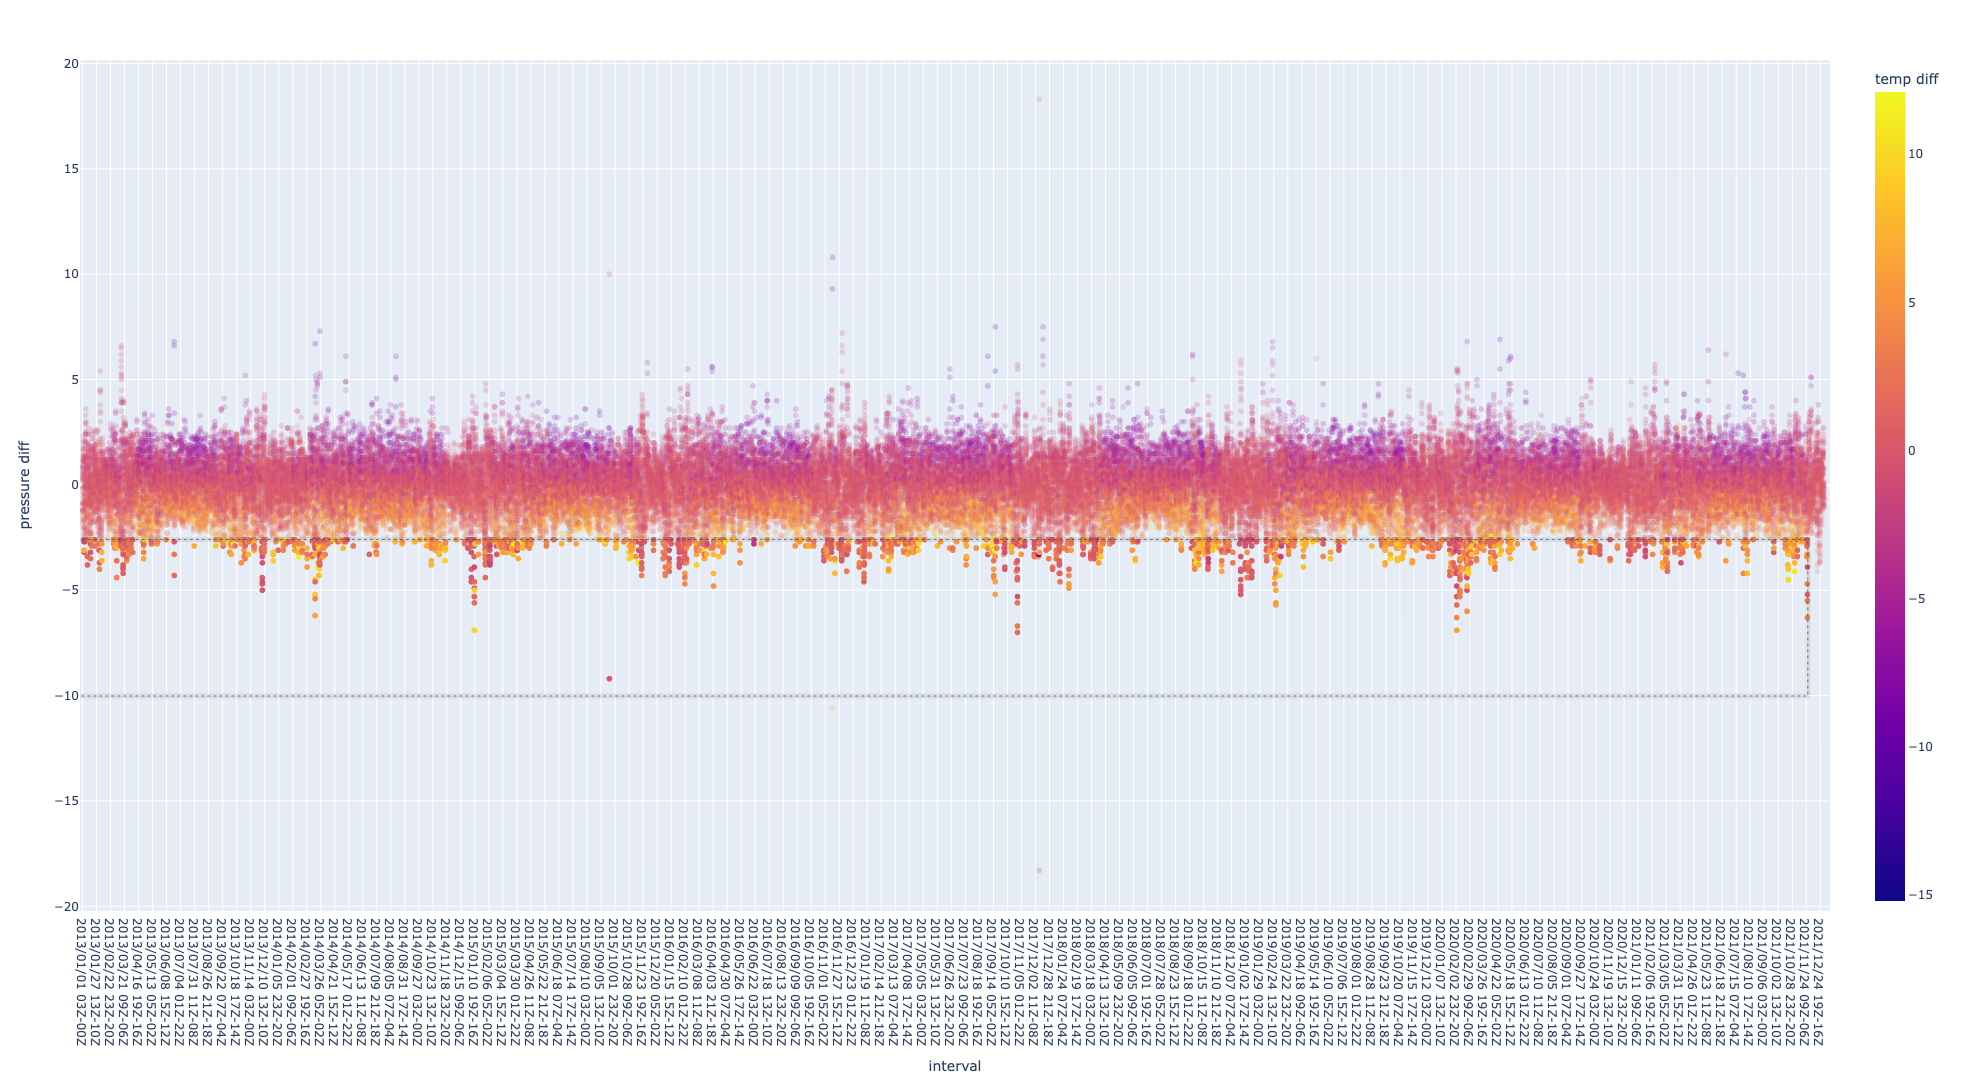
\includegraphics[height=4.6cm]{newplot (3).png}
\caption{Interval [-10, -2.5]}
\label{interval1}

\centering
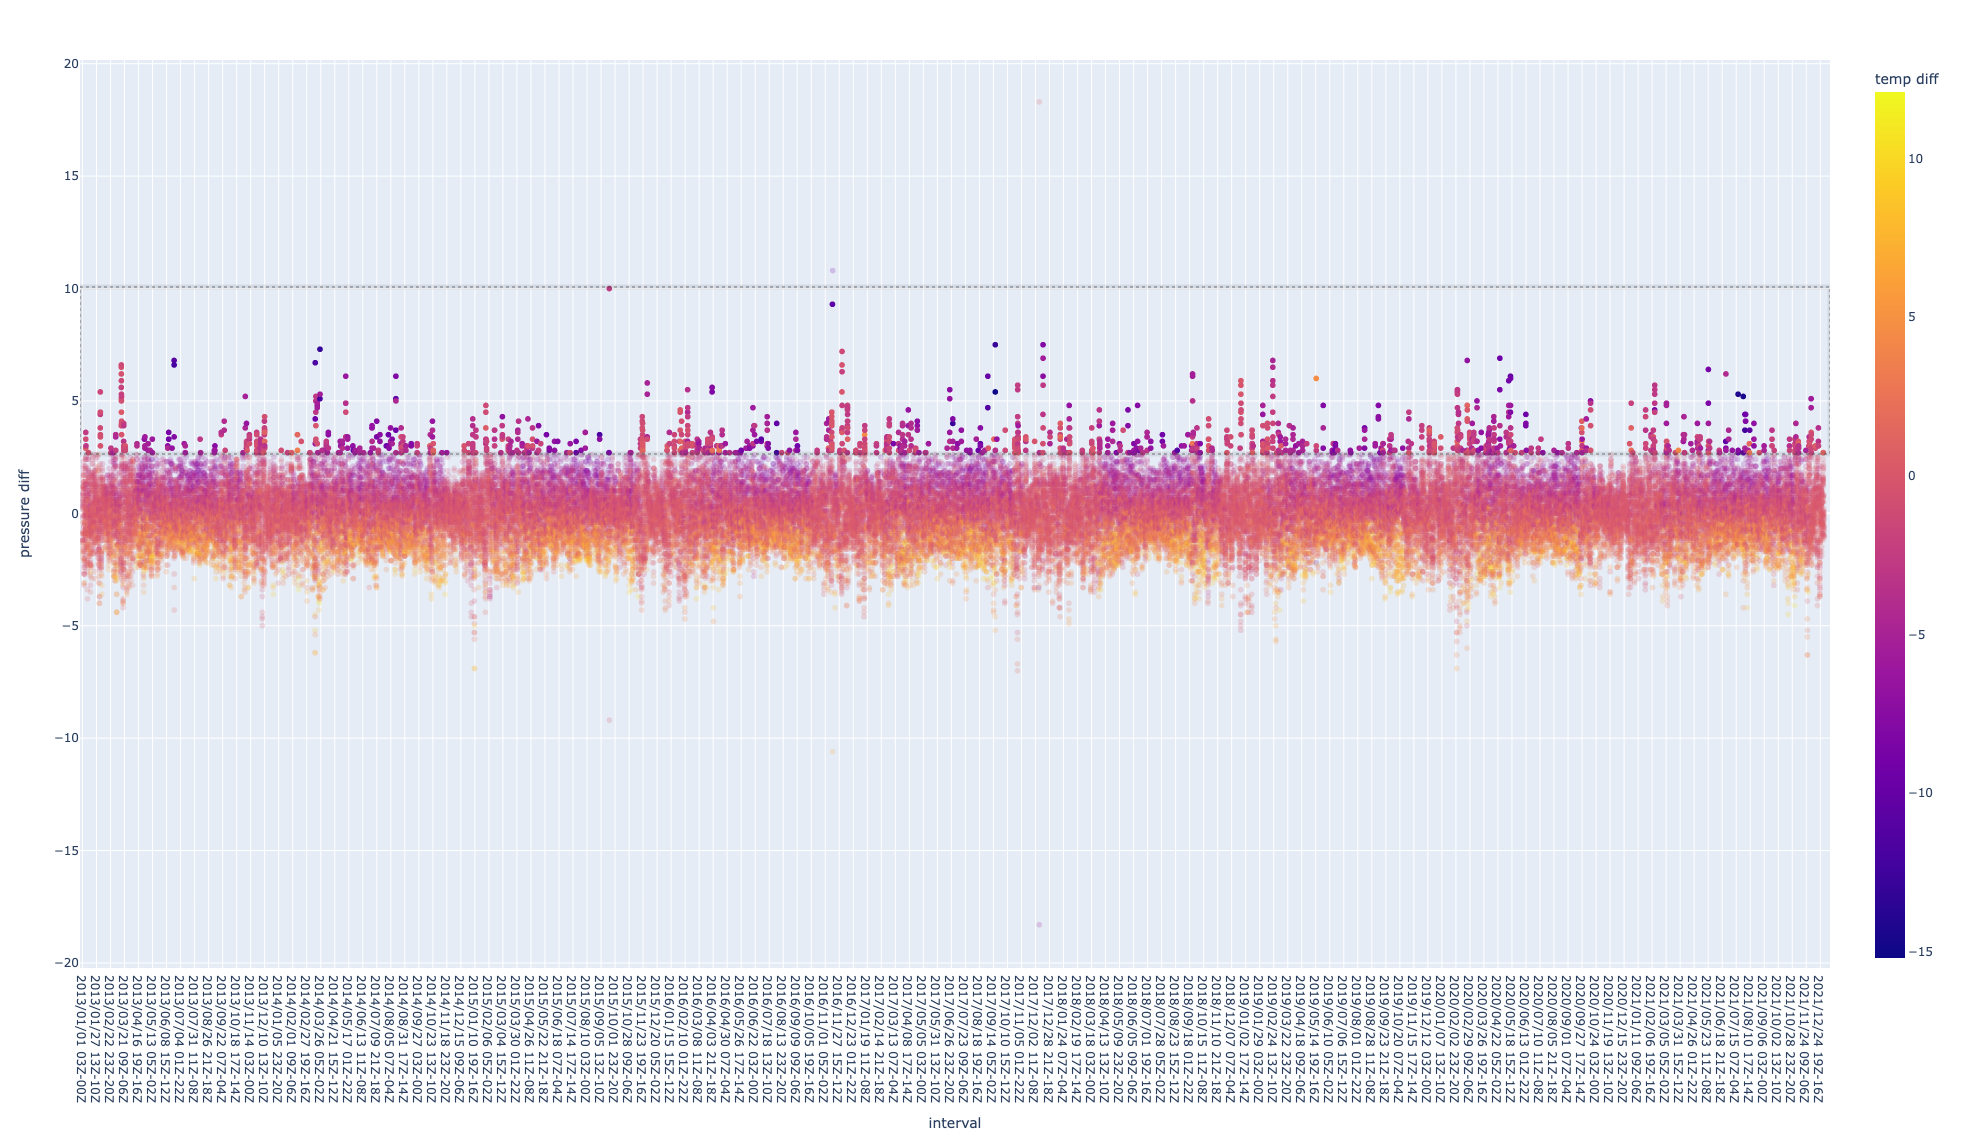
\includegraphics[height=4.6cm]{newplot (2).png}
\caption{Interval [2.5, 10]}
\label{interval2}

\end{multicols}
\end{figure*}

As it can be observed, some of these points have an extreme color for temperature difference as well, so these will be considered critical intervals. Days containing at least one critical interval are considered to be critical days.

\subsection{Data labeling}

The data is automatically labeled with the following approach: every day that has at least one stroke incidence is considered to be critical. The data is loaded from the medical and meteorological datasets and the labeling is done by searching for each day of the 9 years in the medical records. If found, the received label has the value 1, otherwise 0.

\subsection{Experiment and Results}

An Artificial Neural Network is used to classify days in one of the two classes: critical or non-critical. The neural network contains 7 Linear layers with ReLU being used as activation function for each one. The first layer has 120 input channels representing the 120 features of each day (24 differences for each of the 5 parameters) and the last layer has 2 output channels representing the 2 classes: critical and non-critical.
\\

The model is trained with 15 epochs and the datasets are split and shuffled into batches of size 32. This increases the probability for the critical days to be uniformly distributed across batches. 
\\

For each epoch, the train accuracy(\ref{acc}), train loss (\ref{loss}) and test accuracy are computed and plotted. If the current value for the test accuracy is greater than the best one until this iteration, the model is saved as the best one (\ref{confmat}). During the validation phase, a confusion matrix is computed and the one for the best model is also plotted after the training is done. To better visualize the accuracy by classes and observe possible overfitting to one class, the evolution of these values by epochs are also plotted
(\ref{accCl}).
\\

\begin{figure*}[h!] 
\begin{multicols}{2}

\centering
\includegraphics[height=4.5cm]{confmat.png}
\caption{Confusion Matrix} 
\label{confmat}

\centering
\includegraphics[height=4.5cm]{loss.png}
\caption{Train Loss} 
\label{loss}

\centering
\includegraphics[height=4.5cm]{plot4.png}
\caption{Train Accuracy} 
\label{acc}

\centering
\includegraphics[height=4.5cm]{plot5.png}
\caption{Accuracy By Classes} 
\label{accCl}
\end{multicols}
\end{figure*}

Results show a high accuracy, but, as explained in \ref{metrics}, the False Negative values have a high impact on the performance of the model and the Recall is more relevant than the accuracy. In this experiment, the recall is 0, as there is no True Positive prediction. This behavior could appear as a result of a very large dataset with very few examples for positive classification. This is a possible explanation for our experiment as there are less than 70 positive values in more than 3000 records. An improvement could be made by simplifying the input data. The current input has 120 channels containing data about 5 weather parameters in 24 3 hours differences for each day. The input could contain only 5 input channels, one per weather parameter, and its value can be computed as the maximum difference for that parameter during the day. This approach could make a critical day more easily identifiable.

\newpage
\section{Related Work - Comparison}

\subsection{Dataset}

In order to make a relevant comparison between our paper and related work in this field, the dataset used in the experiments must be extended. For this, more meteorological data is collected from multiple weather stations across Transylvania and more medical records are taken into consideration, with the place of the incident being outside of Cluj-Napoca. To put all this data together, every stroke incident must be associated with the closest weather station that provides data for the specific day of the incident. This adds a new processing step that was not needed for the small data set covering Cluj-Napoca only. 

\subsection{Approaches and Metrics}

There are two main approaches for the presented problem in existing literature: statistical calculus and artificial intelligence, most studies using the first one. The data used in each paper is different, as it strongly depends on the geographical area covered by the study. Thus, no comparison can be made between our study and related work on the same data, but overall performance and approaches are relevant even if the input data is different. 
\\

One of the most relevant studies on stroke incidence correlated to weather conditions is by Knezovic et al. The paper is focused on data collected from Zagreb, Croatia, which has a similar climate to Romania, the area observed for the present study. However, the approach in \cite{Knezovic:2018dg} is very different, focusing on statistical methods, with no artificial intelligence involved. Their results show a seasonal variation of stroke occurrence, different per stroke subtype. 
\\

A study with an approach more similar to ours is \cite{Fang:2014dg}. The approach in this paper is centered around a Back Propagation Neural Network (BPNN), so although the used data is different, the methodology is similar, so the results are relevant. Fang et al. obtained a relative error of 6\% for 2010 early January, when the real value was 3.2 and the prediction was 3, a relative error of 7\% for mid January 2010, when the predicted incidence rate was 2.7 and the real one was 2.9. Overall, their predictions had an error between 6\% - 8\% and is considered "accurate and reasonable"(\cite{Fang:2014dg}).


\newpage
\section{Ethics}

No medical data used in the present paper was collected without the consent of the patients and all data is anonymous.

\section{Discussion}
\section{Conclusion}
\newpage

\nocite{*}
\medskip
\begin{multicols}{2}
\printbibliography[heading=bibintoc]
\end{multicols}
\end{document}
